% =============================================
% CHAPITRE 3 : Conception et Architecture du système
% =============================================
\chapter{Conception et Architecture du système}
\label{chap:conception}

\section{Introduction}

Les chapitres précédents ont mis en évidence deux constats~: les attaques \gls{ddos} modernes dépassent les capacités de défense individuelles, et les systèmes collaboratifs existants souffrent d'une centralisation résiduelle ou d'une absence de mécanisme de confiance formalisé. Ce chapitre présente la conception du système distribué de mitigation collaborative qui répond à ces lacunes.

Il est organisé en deux parties~: la \textbf{conception préliminaire} établit les exigences et l'architecture globale du système~; la \textbf{conception technique détaillée} formalise les modèles de données, les algorithmes et les protocoles de sécurité retenus.

% ==================================================
\section{Conception préliminaire}
\label{sec:conception_prelim}
% ==================================================

\subsection{Architecture générale}
\label{sec:architecture_gen}

\subsubsection{Topologie de la coalition}
La solution proposée adopte une architecture \gls{p2p} non structurée, dans laquelle chaque nœud maintient localement un registre des pairs qu'il connaît. Ce choix repose sur trois motivations principales. Premièrement, les participants de la coalition présentent une forte hétérogénéité en termes de ressources et de capacités ; une architecture plate permet ainsi d'éviter la désignation arbitraire de nœuds privilégiés ou de points de concentration. Deuxièmement, cette approche renforce la résilience du système : la défaillance ou le retrait d'un pair n'entraîne pas l'interruption du fonctionnement global du réseau, aucun nœud ne constituant un point central de dépendance. Enfin, elle favorise l'évolutivité de la coalition : de nouveaux participants peuvent rejoindre le réseau sans nécessiter de reconfiguration globale ni de coordination centralisée, permettant ainsi à l'infrastructure de s'adapter progressivement à l'augmentation du nombre de membres \cite{lua2005survey}.

\begin{figure}[H]
\centering
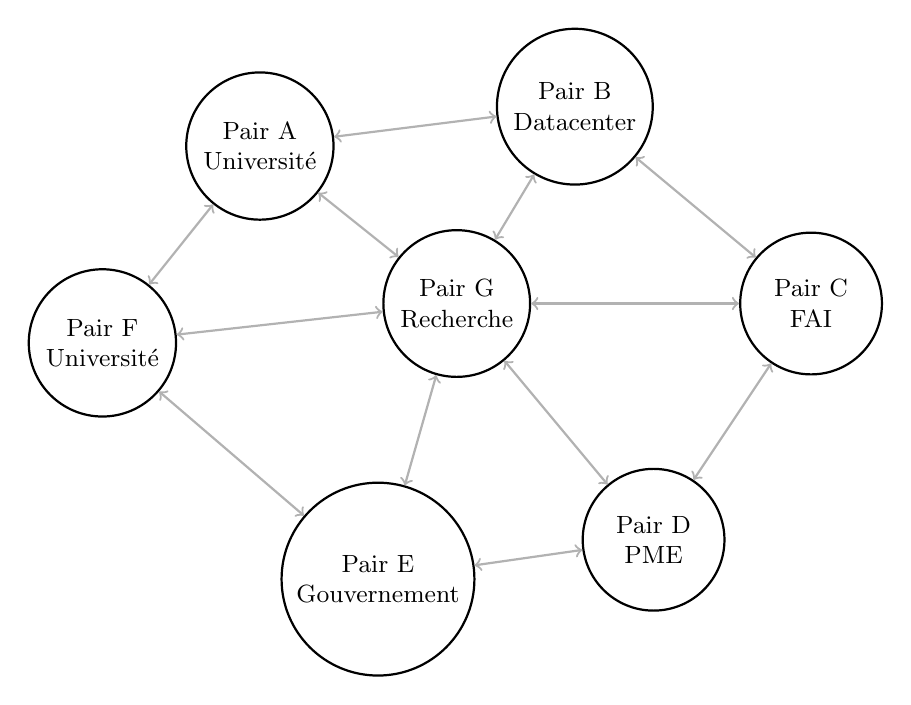
\begin{tikzpicture}[
    pair/.style={
        circle, draw, thick,
        minimum size=1.8cm,
        align=center, font=\small
    },
    lien/.style={<->, thick, gray!60}
]
\node[pair, fill=white]    (A) at (0,3.5)     {Pair A\\Université};
\node[pair, fill=white]   (B) at (4,4)       {Pair B\\Datacenter};
\node[pair, fill=white]  (C) at (7,1.5)     {Pair C\\FAI};
\node[pair, fill=white]  (D) at (5,-1.5)    {Pair D\\PME};
\node[pair, fill=white]     (E) at (1.5,-2)    {Pair E\\Gouvernement};
\node[pair, fill=white]  (F) at (-2,1)      {Pair F\\Université};
\node[pair, fill=white]    (G) at (2.5,1.5)   {Pair G\\Recherche};

\draw[lien] (A) -- (B);
\draw[lien] (B) -- (C);
\draw[lien] (C) -- (D);
\draw[lien] (D) -- (E);
\draw[lien] (E) -- (F);
\draw[lien] (F) -- (A);
\draw[lien] (A) -- (G);
\draw[lien] (B) -- (G);
\draw[lien] (G) -- (D);
\draw[lien] (G) -- (E);
\draw[lien] (F) -- (G);
\draw[lien] (C) -- (G);
\end{tikzpicture}
\caption{Exemple de coalition~: sept nœuds hétérogènes interconnectés en overlay \gls{p2p} plat non structuré.}
\label{fig:coalition}
\end{figure}

\subsubsection{Cycle de vie d'une session de mitigation}
\label{subsec:cycle_vie}

Le flux d'une session d'aide suit quatre phases distinctes~:

\begin{enumerate}
    \item \textbf{Détection et escalade~:} le nœud victime détecte un débordement de capacité et diffuse une demande d'aide à l'ensemble des membres actifs de la coalition, sans présélection ni allocation préalable.
    \item \textbf{Négociation~:} les pairs reçoivent la demande d'aide et acceptent ou rejettent en fonction de leur capacité disponible~; en cas d'acceptation, chaque pair déclare lui-même le volume qu'il peut offrir.
    \item \textbf{Allocation~:} une fois les réponses connues, le nœud victime calcule par l'algorithme WSM la répartition optimale du flux excédentaire parmi les seuls pairs ayant accepté.
    \item \textbf{Redirection active~:} le trafic excédentaire est redirigé vers les pairs acceptants via un tunnel (GRE, VXLAN ou IPIP), selon le plan d'allocation calculé.
    \item \textbf{Clôture~:} à la fin de l'attaque, le nœud victime notifie la clôture ({POST /attack/over}), capture les crédibilités réseau au moment de la session et recalcule les scores de confiance.
\end{enumerate}

\subsection{Périmètre du système}
\label{subsec:perimetre_redirection}

La Figure~\ref{fig:archi_redirection} présente l'architecture globale du système 
et délimite explicitement son périmètre. Le système gère l'intégralité de la 
coordination applicative~: diffusion des demandes d'aide \textbf{(1)}, collecte 
des réponses des pairs acceptants ou refusants \textbf{(2)} et émission du signal 
de redirection \textbf{(3)}. En revanche, la redirection physique du trafic reste 
hors périmètre et repose sur l'infrastructure réseau du nœud victime~: c'est elle qui achemine le trafic excédentaire vers les 
pairs aidants \textbf{(4)}, lesquels filtrent le trafic malveillant et renvoient 
le trafic propre vers cette même infrastructure \textbf{(5)}, avant qu'il ne soit 
agrégé et retransmis au nœud victime \textbf{(6)}.

\begin{figure}[H]
\centering
\figborder[\textwidth]{figures/archi_redirection.pdf}
\caption{Architecture globale du système ShieldNet~: périmètre applicatif et redirection réseau hors périmètre.}
\label{fig:archi_redirection}
\end{figure}

\subsection{Diagrammes de cas d'utilisation}
\label{subsec:uc}

Le système est décrit par trois diagrammes de cas d'utilisation complémentaires, couvrant respectivement le protocole de mitigation collaborative, le moteur de confiance PeerTrust et le rôle complet du nœud pair dans la coalition. Les trois acteurs impliqués sont~: le \textbf{nœud local} (victime en situation d'attaque) et le \textbf{nœud pair} (participant distant).
%et l'\textbf{administrateur} (responsable de la configuration locale).

% --------------------------------------------------
\subsubsection{Protocole de mitigation collaborative}
% --------------------------------------------------
La Figure~\ref{fig:uc_mitigation} détaille les interactions entre le nœud victime 
et le nœud pair lors d'une session de mitigation. Ce diagramme couvre le flux complet 
depuis l'envoi de la demande d'aide jusqu'au recalcul du score de confiance.

Le nœud victime initie la séquence en diffusant une demande d'aide à l'ensemble
des pairs actifs de la coalition, sans présélection ni allocation préalable.
Chaque nœud pair sollicité peut alors accepter ou rejeter la session ; en cas
d'acceptation, il déclare lui-même la capacité qu'il peut offrir. Une fois les
réponses connues, le nœud victime calcule la répartition optimale du flux parmi
les seuls pairs ayant accepté, via l'algorithme WSM : chaque pair accepteur est
évalué selon quatre critères pondérés (capacité déclarée à l'acceptation, latence
inversée, score de confiance et réciprocité). L'acceptation déclenche ensuite
l'activation de la mitigation, qui correspond au signal de démarrage de la
redirection au niveau applicatif. La clôture de l'attaque, initiée par le nœud
victime, inclut deux actions systématiques : la mise à jour des crédits de
réciprocité des deux nœuds dans leurs registres respectifs, et le recalcul du
score de confiance PeerTrust $T(u)$ du pair assistant.

\begin{figure}[H]
\centering
\figborder[\textwidth]{figures/uc_mitigation_collaborative1.pdf}

\caption{Diagramme de cas d'utilisation~: Protocole de mitigation collaborative.}
\label{fig:uc_mitigation}
\end{figure}

% --------------------------------------------------
\subsubsection{Moteur de confiance PeerTrust}
% --------------------------------------------------
La figure~\ref{fig:uc_trust} présente les cas d'utilisation du moteur
de confiance. L'acteur unique est le nœud local, qui peut
déclencher le recalcul du score à la clôture d'une session d'aide,
consulter le score d'un pair, ou forcer un recalcul manuel. Le
bannissement automatique est déclenché lorsque le score calculé
est inférieur à $0{,}20$, ou suite à la détection d'une violation
de comportement.


\begin{figure}[H]
\centering
\figborder[\textwidth]{figures/uc_moteur_confiance.pdf}
\caption{Diagramme de cas d'utilisation~: Moteur de confiance PeerTrust.}
\label{fig:uc_trust}
\end{figure}

% --------------------------------------------------
\subsubsection{Rôle du nœud pair dans la coalition}
% --------------------------------------------------

La Figure~\ref{fig:uc_pair} présente l'ensemble des actions qu'un \textbf{nœud pair} peut effectuer au sein de la coalition, organisées en quatre groupes fonctionnels.

Le groupe \textbf{Membership} couvre le cycle de vie complet du pair~: il s'enregistre, action qui inclut obligatoirement la publication de ses capacités de scrubbing; il peut ensuite découvrir des pairs disponibles et consulter la liste des pairs connus; il diffuse un heartbeat sur événement (adhésion, mise à jour de paramètres ou départ) pour signaler sa disponibilité et mettre à jour sa capacité déclarée~; enfin, il peut quitter proprement la coalition, ce qui met son statut à {INACTIVE} ou {MAINTENANCE}.

Le groupe \textbf{Session d'aide} couvre les deux modes de participation~: le pair peut recevoir une requête d'aide  et choisir de l'accepter  ou de la rejeter , ou bien proposer proactivement de l'aide  lorsque le flag {auto\_offer\_enabled} est activé dans sa politique locale~; une offre acceptée étend vers le même cas d'usage Accepter la session d'aide.

Le groupe \textbf{Confiance} contient un seul cas d'usage~: interroger la coalition sur sa réputation, qui correspond à la collecte de la crédibilité $Cr$ utilisée dans la formule PeerTrust.

Le groupe \textbf{Sécurité} couvre l'obtention d'un token, prérequis à tout appel API authentifié.

\begin{figure}[H]
\centering
\figborder[\textwidth]{figures/uc_role_pair.pdf}
\caption{Diagramme de cas d'utilisation~: Rôle du nœud pair dans la coalition (12 cas d'usage).}
\label{fig:uc_pair}
\end{figure}

% --------------------------------------------------
\subsection{Documentation des cas d'utilisation}
\label{subsec:cu_doc}
% --------------------------------------------------

Les tableaux suivants documentent les six principaux cas d'utilisation du système, issus des trois diagrammes présentés ci-dessus. Le Tableau~\ref{tab:cu_identification} en présente la synthèse.

\begin{comment}
\begin{table}[H]
\centering
\caption{Identification des cas d'utilisation.}
\label{tab:cu_identification}
\small
\renewcommand{\arraystretch}{1.35}
\begin{tabularx}{\textwidth}{|c|l|l|X|}
\hline
\textbf{ID} & \textbf{Nom} & \textbf{Acteur principal} & \textbf{Description courte} \\
\hline
CU~1 & Obtenir un token JWT RS256      & Nœud local / pair      & Authentification auprès de l'API via une clé privée RS256~; token valable 15~minutes. \\
\hline
CU~3 & Envoyer un heartbeat            & Nœud pair              & Signal périodique (30~s) transmettant la charge et la capacité disponible. \\
\hline
CU~4 & Envoyer une requête d'aide      & Nœud victime           & Sélection WSM des pairs et envoi de {POST /help/request}. \\
\hline
CU~5 & Accepter ou rejeter une session & Nœud pair              & Réponse à une requête d'aide selon la capacité disponible. \\
\hline
CU~6 & Clôturer l'attaque              & Nœud victime           & Fermeture des sessions, mise à jour des crédits et recalcul PeerTrust. \\
\hline
CU~7 & Recalculer le score PeerTrust   & Moteur de confiance    & Calcul de $T(u)$ et bannissement automatique si $T(u) < 0{,}20$. \\
\hline
\end{tabularx}
\end{table}
\end{comment}


\begin{table}[H]
\centering
\caption{Identification des cas d'utilisation.}
\label{tab:cu_identification}

\renewcommand{\arraystretch}{1.8}
\setlength{\tabcolsep}{5pt}

\begin{tabular}{|
>{\raggedright\arraybackslash}p{1.2cm}|
>{\raggedright\arraybackslash}p{3.5cm}|
>{\raggedright\arraybackslash}p{3.0cm}|
>{\raggedright\arraybackslash}p{5.0cm}|}
\hline

\textbf{ID} &
\textbf{Nom} &
\textbf{Acteur principal} &
\textbf{Description courte} \\
\hline

CU~1 &
Obtenir un token JWT RS256 &
Nœud local / pair &
Authentification auprès de l'API via une clé privée RS256 ; token valable 15~m. \\
\hline

CU~3 &
Envoyer un heartbeat &
Nœud pair &
Signal événementiel (adhésion, mise à jour ou départ) transmettant la charge et la capacité disponible. \\
\hline

CU~4 &
Envoyer une requête d'aide &
Nœud victime &
Sollicitation diffusée à tous les pairs actifs, sans allocation préalable. \\
\hline

CU~5 &
Accepter ou rejeter une session &
Nœud pair &
Réponse à une requête d'aide, avec déclaration de la capacité offerte. \\
\hline

CU~5bis &
Calculer l'allocation WSM &
Nœud victime &
Répartition optimale du flux entre les pairs ayant accepté. \\
\hline

CU~6 &
Clôturer l'attaque &
Nœud victime &
Fermeture des sessions, mise à jour des crédits et recalcul PeerTrust. \\
\hline

CU~7 &
Recalculer le score PeerTrust &
Moteur de confiance &
Calcul de $T(u)$ et bannissement automatique si $T(u) < 0{,}20$. \\
\hline

\end{tabular}

\end{table}



% ─── CU 1 ─────────────────────────────────────────────────────────────────────
\begin{table}[H]
\centering
\renewcommand{\arraystretch}{1.5}
\begin{tabular}{|p{3.5cm}|p{10.5cm}|}
\hline
\multicolumn{2}{|c|}{\textbf{CU~1 : Obtenir un token JWT RS256}} \\
\hline
\textbf{ID} & 1 \\
\hline
\textbf{Description} & Le nœud (local ou pair) demande un token JWT signé RS256 afin d'accéder aux routes protégées de l'API. Le token est valide exactement 15~minutes. \\
\hline
\textbf{Acteurs primaires} & Nœud local, nœud pair \\
\hline
\textbf{Acteurs secondaires} & Module d'authentification (composant interne du nœud cible) \\
\hline
\textbf{Préconditions} & La clé privée RSA du nœud ({node.key}) est présente sur le système de fichiers. \\
\hline
\textbf{Enchaînement principal} &
Ce CU démarre lorsque le nœud doit appeler une route protégée de l'API.\newline
\textbf{1.}\ Le nœud envoie {POST /api/v1/auth/token} avec son identifiant ({node\_id}).\newline
\textbf{2.}\ Le module d'authentification lit la clé privée RS256 stockée localement ({node.key}).\newline
\textbf{3.}\ Le système génère un JWT signé contenant {\{iss, node\_id, iat, exp\}} avec une durée de vie de 15~minutes.\newline
\textbf{4.}\ Le token est retourné au nœud appelant (HTTP~200).\newline
\textbf{5.}\ Le nœud inclut ce token dans l'en-tête {Authorization: Bearer <token>} pour toutes ses requêtes suivantes. \\
\hline
\textbf{Post-conditions} & Le nœud dispose d'un token RS256 valide pour 15~minutes. \\
\hline
\textbf{Enchaînements alternatifs} &
\textbf{Clé privée introuvable~:} le serveur retourne HTTP~500.\newline
\textbf{Token expiré lors d'un appel ultérieur~:} le serveur retourne HTTP~401 ; le nœud doit redemander un token via ce même CU. \\
\hline
\end{tabular}
\caption{Documentation du cas d'utilisation \textit{Obtenir un token JWT RS256}.}
\label{tab:cu1}
\end{table}


% ─── CU 3 ─────────────────────────────────────────────────────────────────────
\begin{table}[H]
\centering
\renewcommand{\arraystretch}{1.5}
\begin{tabular}{|p{3.5cm}|p{10.5cm}|}
\hline
\multicolumn{2}{|c|}{\textbf{CU~3 : Envoyer un heartbeat}} \\
\hline
\textbf{ID} & 3 \\
\hline
\textbf{Description} & Un nœud pair signale sa disponibilité et met à jour sa capacité déclarée auprès de ses pairs connus, sur événement uniquement~: aucun minuteur périodique n'envoie de signal en l'absence de changement. \\
\hline
\textbf{Acteurs primaires} & Nœud pair \\
\hline
\textbf{Acteurs secondaires} & Nœuds pairs connus (registres distants de la coalition) \\
\hline
\textbf{Préconditions} & Le nœud pair est enregistré (statut \texttt{ACTIVE}). \\
\hline
\textbf{Enchaînement principal} &
Ce CU est déclenché par l'un des trois événements suivants~: adhésion à la coalition, mise à jour de ses propres paramètres (capacité, charge) ou départ propre de la coalition.\newline
\textbf{1.}\ Le pair diffuse {POST /heartbeat} à chacun de ses pairs connus, avec~: son identifiant, son statut, sa charge courante ({reported\_load\_pct}) et sa capacité disponible ({reported\_available\_gbps}).\newline
\textbf{2.}\ Chaque pair destinataire met à jour le champ {last\_heartbeat} et la capacité déclarée de l'émetteur.\newline
\textbf{3.}\ Si une attaque est en cours côté destinataire, la réception du heartbeat déclenche une reconsidération de la coalition (cf.\ CU~5bis) afin de tenir compte de la capacité mise à jour.\newline
\textbf{4.}\ Le destinataire retourne HTTP~201 avec confirmation d'enregistrement. \\
\hline
\textbf{Post-conditions} & {last\_heartbeat} et la capacité déclarée du pair émetteur sont à jour chez chaque destinataire~; la coalition est reconsidérée si une attaque est en cours. \\
\hline
\textbf{Enchaînements alternatifs} &
\textbf{Pair banni ou inconnu~:} le nœud retourne HTTP~403 (Forbidden) ou 404.\newline
\textbf{Pair injoignable lors de la diffusion~:} l'échec est journalisé sans marquage automatique~; la détection de panne est réactive (cf.\ CU~4), déclenchée uniquement par l'échec d'une vraie sollicitation, jamais par l'absence de heartbeat. \\

\hline
\end{tabular}
\caption{Documentation du cas d'utilisation \textit{Envoyer un heartbeat}.}
\label{tab:cu3}
\end{table}

% ─── CU 4 ─────────────────────────────────────────────────────────────────────



\begin{table}[H]
\centering
\renewcommand{\arraystretch}{1.5}
\begin{tabular}{|p{3.5cm}|p{10.5cm}|}
\hline
\multicolumn{2}{|c|}{\textbf{CU~4 : Envoyer une requête d'aide (sollicitation diffusée)}} \\
\hline
\textbf{ID} & 4 \\
\hline
\textbf{Description} & Le nœud victime, confronté à une congestion dépassant sa capacité locale, sollicite l'ensemble des pairs actifs de la coalition~: à ce stade, aucune sélection ni allocation n'est encore calculée — la demande se limite à interroger la disponibilité de chacun. \\
\hline
\textbf{Acteurs primaires} & Nœud victime (nœud local sous attaque) \\
\hline
\textbf{Acteurs secondaires} & Nœuds pairs candidats \\
\hline
\textbf{Préconditions} & Le nœud victime est authentifié (CU~1)~; au moins un pair est en statut {ACTIVE} dans la coalition. \\
\hline
\textbf{Enchaînement principal} &
Ce CU démarre lorsque la congestion détectée dépasse la capacité de filtrage locale du nœud.\newline
\textbf{1.}\ Le nœud victime récupère la liste des pairs en statut {ACTIVE} ({GET /api/v1/peers}).\newline
\textbf{2.}\ Le nœud victime envoie {POST /api/v1/help/request} à \emph{chacun} de ces pairs, la requête se limite à {attack\_id} et {helping\_peer\_id}.\newline
\textbf{3.}\ La session passe immédiatement au statut {OFFERED} chez le pair. \\
\hline
\textbf{Post-conditions} & Une session est créée pour chaque pair sollicité, en statut {OFFERED}, {ACCEPTED} ou {REJECTED}~; aucune allocation n'est encore déterminée à ce stade. \\
\hline
\textbf{Enchaînements alternatifs} &
\textbf{Aucun pair {ACTIVE} dans la coalition~:} la liste est vide~; le nœud victime gère l'attaque seul.\newline
\textbf{Pair banni ou expulsé~:} la sollicitation est rejetée (HTTP~403) avant création de session. \\
\hline
\end{tabular}
\caption{Documentation du cas d'utilisation \textit{Envoyer une requête d'aide (sollicitation diffusée)}.}
\label{tab:cu4}
\end{table}

% ─── CU 5bis ──────────────────────────────────────────────────────────────────
\begin{table}[H]
\centering
\renewcommand{\arraystretch}{1.5}
\begin{tabular}{|p{3.5cm}|p{10.5cm}|}
\hline
\multicolumn{2}{|c|}{\textbf{CU~5bis : Calculer l'allocation WSM}} \\
\hline
\textbf{ID} & 5b \\
\hline
\textbf{Description} & Une fois les réponses des pairs sollicités connues, le nœud victime calcule la répartition optimale du flux excédentaire parmi les seuls pairs ayant accepté, à l'aide de l'algorithme WSM. \\
\hline
\textbf{Acteurs primaires} & Nœud victime \\
\hline
\textbf{Acteurs secondaires} & Aucun (calcul local, base de données uniquement) \\
\hline
\textbf{Préconditions} & Au moins une session est en statut {ACCEPTED} pour l'attaque considérée (CU~5). \\
\hline
\textbf{Enchaînement principal} &
Ce CU démarre lorsque le nœud victime juge avoir reçu suffisamment de réponses (CU~5) pour planifier la mitigation.\newline
\textbf{1.}\ Le nœud victime appelle {POST /api/v1/attack/\{id\}/allocate}.\newline
\textbf{2.}\ Le système restreint le calcul WSM aux seuls pairs en statut {ACCEPTED} pour cette attaque, en utilisant pour chacun la capacité qu'il a déclarée à l'acceptation ({accepted\_volume\_gbps}) comme critère $C_p$ — et non plus l'ancienne capacité issue du dernier heartbeat.\newline
\textbf{3.}\ Le système calcule pour chacun le score pondéré~:\newline
\quad $\text{Score}(p) = 0{,}545 \cdot C_p + 0{,}193 \cdot L_p + 0{,}193 \cdot T_p + 0{,}069 \cdot R_p$\newline
\textbf{4.}\ Le système calcule le poids $w_i = \text{Score}(p_i) / \sum_j \text{Score}(p_j)$ et l'allocation {allocation\_pct} de chaque session acceptée (Éq.~\ref{eq:alloc}).\newline
\textbf{5.}\ Le champ {allocation\_pct} de chaque session {ACCEPTED} est mis à jour avec le résultat. \\
\hline
\textbf{Post-conditions} & Chaque session {ACCEPTED} porte désormais une {allocation\_pct} calculée, prête pour l'activation (CU~6). \\
\hline
\textbf{Enchaînements alternatifs} &
\textbf{Aucune session {ACCEPTED}~:} le système retourne une liste vide ; le nœud victime gère l'attaque avec sa seule capacité locale.\newline
\textbf{Nouvelle acceptation après un premier calcul~:} ce CU peut être rappelé pour recalculer le plan sur l'ensemble mis à jour des accepteurs. \\
\hline
\end{tabular}
\caption{Documentation du cas d'utilisation \textit{Calculer l'allocation WSM}.}
\label{tab:cu5bis}
\end{table}






% ─── CU 5 ─────────────────────────────────────────────────────────────────────
\begin{table}[H]
\centering
\renewcommand{\arraystretch}{1.5}
\begin{tabular}{|p{3.5cm}|p{10.5cm}|}
\hline
\multicolumn{2}{|c|}{\textbf{CU~5 : Accepter ou rejeter une session d'aide}} \\
\hline
\textbf{ID} & 5 \\
\hline
\textbf{Description} & Un nœud pair, ayant reçu une requête d'aide (CU~4) sans volume ni allocation imposés, évalue sa propre disponibilité et accepte ou rejette la session en déclarant lui-même la capacité qu'il peut offrir. \\
\hline
\textbf{Acteurs primaires} & Nœud pair \\
\hline
\textbf{Acteurs secondaires} & Nœud victime \\
\hline
\textbf{Préconditions} & Une session d'aide en statut {OFFERED} est associée au pair~; le pair est authentifié (CU~1). \\
\hline
\textbf{Enchaînement principal} &
Ce CU démarre dès réception d'une requête {POST /help/request} par le nœud pair.\newline
\textbf{1.}\ Le pair consulte sa capacité disponible courante ({reported\_available\_gbps}) et sa charge actuelle ({reported\_load\_pct}) — la requête reçue ne lui impose aucun volume cible.\newline
\textbf{2.}\ S'il peut contribuer~:\newline
\quad \textbf{*}\ Le pair envoie {PUT /api/v1/help/\{id\}/accept} en déclarant lui-même la capacité qu'il offre ({accepted\_volume\_gbps})~; la session passe en statut {ACCEPTED}.\newline
\quad \textbf{*}\ Le nœud victime est notifié~; cette capacité servira de critère $C_p$ au calcul d'allocation WSM (CU~5bis).\newline
\textbf{3.}\ S'il ne peut pas contribuer~:\newline
\quad \textbf{*}\ Le pair envoie {PUT /api/v1/help/\{id\}/reject}~; la session passe en statut {REJECTED}.\newline
\quad \textbf{*}\ Le nœud victime est notifié du refus et poursuit avec les autres pairs sollicités. \\
\hline
\textbf{Post-conditions} & La session est en statut {ACCEPTED} (avec {accepted\_volume\_gbps} renseigné) ou {REJECTED}~; le nœud victime est informé de la décision. \\
\hline
\textbf{Enchaînements alternatifs} &
\textbf{Session déjà traitée (statut non {OFFERED})~:} le nœud retourne HTTP~409 (Conflict).\newline
\textbf{Token JWT expiré~:} le nœud retourne HTTP~401. \\
\hline
\end{tabular}
\caption{Documentation du cas d'utilisation \textit{Accepter ou rejeter une session d'aide}.}
\label{tab:cu5}
\end{table}

% ─── CU 6 ─────────────────────────────────────────────────────────────────────
\begin{table}[H]
\centering
\renewcommand{\arraystretch}{1.5}
\begin{tabular}{|p{3.5cm}|p{10.5cm}|}
\hline
\multicolumn{2}{|c|}{\textbf{CU~6 : Clôturer l'attaque}} \\
\hline
\textbf{ID} & 6 \\
\hline
\textbf{Description} & À la fin de l'attaque DDoS, le nœud victime clôture la session d'aide, met à jour les crédits de réciprocité des deux nœuds et déclenche le recalcul du score de confiance PeerTrust de chaque pair assistant. \\
\hline
\textbf{Acteurs primaires} & Nœud victime \\
\hline
\textbf{Acteurs secondaires} & Nœuds pairs assistants, moteur de confiance PeerTrust \\
\hline
\textbf{Préconditions} & Au moins une session d'aide est en statut \texttt{ACTIVE}~;
le nœud victime est authentifié (CU~1). \\

\hline
\textbf{Enchaînement principal} &
Ce CU démarre lorsque le nœud victime détecte la fin de l'attaque DDoS.\newline
\textbf{1.}\ Le nœud victime envoie {POST /api/v1/attack/over} avec le {session\_id} et le volume réellement traité par le pair ({actual\_volume\_gbps}).\newline
\textbf{2.}\ Le système calcule le ratio de satisfaction $S = \min(1{,}0,\ \textit{réel} / \textit{accepté})$ pour chaque pair assistant.\newline
\textbf{3.}\ Les crédits de réciprocité sont mis à jour dans les ledgers respectifs du nœud victime et du pair assistant.\newline
\textbf{4.}\ Le moteur de confiance recalcule le score PeerTrust $T(u)$ de chaque pair assistant (CU~7).\newline
\textbf{5.}\ La session est marquée {COMPLETED}. \\
\hline
\textbf{Post-conditions} & Session en statut {COMPLETED}~; scores de confiance et crédits de réciprocité mis à jour. \\
\hline
\textbf{Enchaînements alternatifs} &
\textbf{Session introuvable~:} le système retourne HTTP~404.\newline
\textbf{Volume réel nul ($S = 0$, pair n'a rien traité)~:} le score PeerTrust chute~; si $T(u) < 0{,}20$, le bannissement automatique est déclenché (CU~7). \\
\hline
\end{tabular}



\caption{Documentation du cas d'utilisation \textit{Clôturer l'attaque}.}
\label{tab:cu6}
\end{table}

% ─── CU 7 ─────────────────────────────────────────────────────────────────────
\begin{table}[H]
\centering
\renewcommand{\arraystretch}{1.5}
\begin{tabular}{|p{3.5cm}|p{10.5cm}|}
\hline
\multicolumn{2}{|c|}{\textbf{CU~7 : Recalculer le score PeerTrust (bannissement automatique)}} \\
\hline
\textbf{ID} & 7 \\
\hline
\textbf{Description} & Le moteur de confiance recalcule le score PeerTrust $T(u)$ d'un pair à partir de l'historique de ses interactions. Si $T(u) < 0{,}20$, le bannissement automatique est déclenché. \\
\hline
\textbf{Acteurs primaires} & Moteur de confiance (système) \\
\hline
\textbf{Acteurs secondaires} & Pair évalué. \\
\hline
\textbf{Préconditions} & Au moins une interaction du pair est enregistrée en base~; ce CU est inclus par CU~6 ou déclenché manuellement via {POST /api/v1/trust/\{id\}/recalculate}. \\
\hline
\textbf{Enchaînement principal} &
Ce CU démarre automatiquement à la clôture d'une session (CU~6) ou sur demande explicite.\newline
\textbf{1.}\ Le système lit l'historique des sessions complétées du pair en base.
La valeur $Cr_i$ de chaque session est lue depuis le champ \texttt{cr\_value}
enregistré à la clôture de cette session (CU~6).\newline

\textbf{2.}\ Le système calcule le score PeerTrust selon la formule de Xiong \& Liu~(2004)~:\newline
\quad $T(u) = \displaystyle\sum_i [S_i \cdot Cr_i \cdot D_i] \;\big/\; \displaystyle\sum_i [Cr_i \cdot D_i]$\newline
où $S_i = \min(1,\ \textit{réel}_i / \textit{accepté}_i)$ et $D_i$ est le poids de sévérité de l'attaque.\newline
\textbf{3.}\ Le niveau de confiance est mis à jour selon les seuils~:\newline
\quad \textbf{*}\ $T(u) \geq 0{,}80$ : niveau {GOLD}\newline
\quad \textbf{*}\ $T(u) \geq 0{,}60$ : niveau {SILVER}\newline
\quad \textbf{*}\ $T(u) \geq 0{,}40$ : niveau {BRONZE}\newline
\quad \textbf{*}\ $T(u) \geq 0{,}20$ : niveau {SUSPECT}\newline
\quad \textbf{*}\ $T(u) < 0{,}20$ : niveau {BANNED} $\rightarrow$ bannissement automatique\newline
\textbf{4.}\ En cas de bannissement~: le statut du pair passe à {BANNED} et son membership à {EXPELLED}. \\
\hline
\textbf{Post-conditions} & Le score $T(u)$ et le niveau de confiance du pair sont persistés en base. \\
\hline
\textbf{Enchaînements alternatifs} &
\textbf{Aucune interaction enregistrée~:} le score reste inchangé à sa valeur initiale ($0{,}50$).\newline \\
\hline
\end{tabular}
\caption{Documentation du cas d'utilisation \textit{Recalculer le score PeerTrust}.}
\label{tab:cu7}
\end{table}

% ==================================================
\section{Conception technique détaillée}
\label{sec:conception_technique}
% ==================================================

\subsection{Modèle de données}
\label{sec:modele_donnees}

Le système adopte un \textbf{modèle de données relationnel}, implémenté via PostgreSQL. Ce choix est motivé par les contraintes propres au système~: les relations entre pairs, sessions d'aide, scores de confiance et transactions de réciprocité forment un graphe d'entités fortement interdépendantes, pour lequel l'intégrité référentielle garantie par les clés étrangères et les contraintes de cascade est indispensable. Les types natifs de PostgreSQL ({UUID}, {ENUM}, {FLOAT}) et le support des transactions ACID assurent de plus la cohérence des scores calculés lors des clôtures de sessions concurrentes. À l’inverse, un modèle non relationnel, orienté document ou clé-valeur, aurait nécessité la mise en œuvre de mécanismes supplémentaires pour assurer le même niveau de cohérence et de gestion des relations entre les différentes entités.

\subsubsection{Diagrammes de classes}

La base de données PostgreSQL locale de chaque nœud comporte quatorze tables, réparties en trois groupes fonctionnels~: la configuration du nœud local, la gestion des pairs et de la confiance, et les sessions de mitigation. Ces trois groupes sont représentés par les diagrammes de classes ci-après~; le Tableau~\ref{tab:tables} décrit le rôle de chaque entité.

L'entité centrale est {PEERS}, qui référence les pairs connus de la coalition. Elle est reliée par des suppressions en cascade à {TRUST\_SCORES} (un score agrégé par pair, mis à jour en place), {TRUST\_VIOLATIONS} (historique des comportements anormaux), {HEARTBEAT\_LOG} (signaux de présence), {RECIPROCITY\_LEDGER} (solde crédit/débit unique par pair) et {MESSAGE\_LOG} (journal des échanges, avec une auto-relation pour les messages de réponse). La table {PEER\_CAPABILITIES} complète ce profil avec les capacités déclarées et vérifiées du pair.

Le nœud local est décrit par {LOCAL\_NODE\_CONFIG}, dont dépendent {SCRUBBING\_CAPABILITIES} (capacités techniques de filtrage~: débit maximal, précision de filtrage) et {POLICY\_CONFIG} (paramètres de politique locale avec versioning~: le champ {is\_current} distingue la politique active des versions historiques, permettant de tracer l'évolution de la configuration dans le temps). Les sessions de mitigation sont modélisées par {HELP\_SESSIONS}, reliée à {ATTACKS} par une clé étrangère en cascade, au pair assistant et au nœud demandeur ({LOCAL\_NODE\_CONFIG}) via des contraintes {RESTRICT}. Chaque session peut générer plusieurs transactions dans {RECIPROCITY\_TRANSACTIONS}, liée à la fois à {HELP\_SESSIONS} (SET NULL) et à {PEERS} (CASCADE). Enfin, {AUDIT\_LOG} est une table autonome sans clé étrangère~: ses colonnes {actor} et {target} sont de type texte libre, garantissant la persistance des entrées même après suppression d'un pair.


\begin{comment}
\begin{table}[H]
\centering
\caption{Description des tables de la base de données.}
\label{tab:tables}
\small
\renewcommand{\arraystretch}{1.35}
\begin{tabularx}{\textwidth}{|l|X|}
\hline
\textbf{Table} & \textbf{Rôle} \\
\hline
{LOCAL\_NODE\_CONFIG} & Configuration du nœud local~: identité, organisation, code pays, ASN, URL d'API, clé publique, empreinte de certificat, capacité maximale de scrubbing, charge courante, date d'adhésion à la coalition. \\
\hline
{PEERS} & Registre des pairs connus~: organisation, type d'organisation, code pays, ASN, URL d'API, clé publique, empreinte de certificat, capacité déclarée, latence mesurée, statut de membership et type de relation. \\
\hline
{TRUST\_SCORES} & Score de confiance d'un pair~: score global PeerTrust, niveau (GOLD à BANNED), sous-scores de fiabilité, performance, réciprocité et stabilité, statistiques de sessions et date de dernier calcul. \\
\hline
{ATTACKS} & Journal des attaques détectées~: volume de pointe, volume en débordement, capacité locale au moment de la détection, sévérité, nombre de pairs impliqués, statut et durée. \\
\hline
{HELP\_SESSIONS} & Sessions d'aide inter-nœuds~: nœud demandeur, pair assistant, direction, volumes acceptés et réels, crédits échangés, note de qualité, valeur $Cr$ capturée à la clôture, horodatages des phases clés. \\
\hline
{RECIPROCITY\_LEDGER} & Solde de réciprocité d'un pair~: crédits donnés, reçus et solde net en Gbps cumulés, date de dernière transaction. \\
\hline
{POLICY\_CONFIG} & Paramètres de politique locale avec versioning~: score de confiance minimal requis, pourcentage de capacité partageable, fréquence de heartbeat, activation des offres automatiques, indicateur de version active ({is\_current}). \\
\hline
{TRUST\_VIOLATIONS} & Violations de comportement détectées~: type, sévérité, description, sanction appliquée et date d'expiration de la sanction. \\
\hline
{HEARTBEAT\_LOG} & Historique des signaux de présence reçus des pairs~: statut reporté, charge, capacité disponible et latence aller-retour. \\
\hline
{AUDIT\_LOG} & Journal d'audit immuable~: type d'événement, sévérité, acteur, cible, description horodatée~; sans clé étrangère pour garantir la persistance après suppression d'un pair. \\
\hline
{SCRUBBING\_CAPABILITIES} & Capacités techniques de filtrage du nœud local~: débit maximal en Gbps, précision de filtrage et statut d'activation. \\
\hline
{MESSAGE\_LOG} & Journal des messages échangés entre nœuds~: type, direction, priorité, validité de signature, résultat de traitement, raison de rejet et auto-référence pour les messages de réponse. \\
\hline
{PEER\_CAPABILITIES} & Capacités déclarées d'un pair distant~: capacité en Gbps, statut et date de vérification. \\
\hline
{RECIPROCITY\_TRANSACTIONS} & Journal des transactions de réciprocité~: type, montant en crédits ({credit\_amount}), session associée (nullable), horodatage. \\
\hline
\end{tabularx}
\end{table}
\end{comment}

\renewcommand{\arraystretch}{1.3}

\begin{longtable}{|
>{\raggedright\arraybackslash}p{5.2cm}|
>{\raggedright\arraybackslash}p{10.2cm}|}
\caption{Description des tables de la base de données.}
\label{tab:tables}
\\
\hline
\textbf{Table} & \textbf{Rôle} \\
\hline
\endfirsthead

\hline
\textbf{Table} & \textbf{Rôle} \\
\hline
\endhead

\hline
\multicolumn{2}{r}{\textit{Suite à la page suivante}} \\
\endfoot

\hline
\endlastfoot

\texttt{LOCAL\_NODE\_CONFIG} &
Configuration du nœud local : identité, organisation, code pays, ASN, URL d'API, clé publique, empreinte de certificat, capacité maximale de scrubbing, charge courante et date d'adhésion à la coalition. \\
\hline

\texttt{PEERS} &
Registre des pairs connus : organisation, type d'organisation, code pays, ASN, URL d'API, clé publique, empreinte de certificat, capacité déclarée, latence mesurée, statut de membership et type de relation. \\
\hline

\texttt{TRUST\_SCORES} &
Score de confiance d'un pair : score global PeerTrust, niveau (GOLD à BANNED), sous-scores de fiabilité, performance, réciprocité et stabilité, statistiques de sessions et date du dernier calcul. \\
\hline

\texttt{ATTACKS} &
Journal des attaques détectées : volume de pointe, volume en débordement, capacité locale au moment de la détection, sévérité, nombre de pairs impliqués, statut et durée. \\
\hline

\texttt{HELP\_SESSIONS} &
Sessions d'aide inter-nœuds : nœud demandeur, pair assistant, direction, volumes acceptés et réels, crédits échangés, note de qualité, valeur $Cr$ capturée à la clôture et horodatages des phases clés. \\
\hline

\texttt{RECIPROCITY\_LEDGER} &
Solde de réciprocité d'un pair : crédits donnés, reçus et solde net en Gbps cumulés, avec date de dernière transaction. \\
\hline

\texttt{POLICY\_CONFIG} &
Paramètres de politique locale avec versioning : score de confiance minimal requis, pourcentage de capacité partageable, fréquence des heartbeats, activation des offres automatiques et indicateur de version active (\texttt{is\_current}). \\
\hline

\texttt{TRUST\_VIOLATIONS} &
Violations de comportement détectées : type, sévérité, description, sanction appliquée et date d'expiration de la sanction. \\
\hline

\texttt{HEARTBEAT\_LOG} &
Historique des signaux de présence reçus des pairs : statut reporté, charge, capacité disponible et latence aller-retour. \\
\hline

\texttt{AUDIT\_LOG} &
Journal d'audit immuable : type d'événement, sévérité, acteur, cible et description horodatée, sans clé étrangère afin de garantir la persistance après suppression d'un pair. \\
\hline

\texttt{SCRUBBING\_CAPABILITIES} &
Capacités techniques de filtrage du nœud local : débit maximal en Gbps, précision de filtrage et statut d'activation. \\
\hline

\texttt{MESSAGE\_LOG} &
Journal des messages échangés entre nœuds : type, direction, priorité, validité de signature, résultat de traitement, raison de rejet et auto-référence pour les messages de réponse. \\
\hline

\texttt{PEER\_CAPABILITIES} &
Capacités déclarées d'un pair distant : capacité en Gbps, statut et date de vérification. \\
\hline

\texttt{RECIPROCITY\_TRANSACTIONS} &
Journal des transactions de réciprocité : type, montant en crédits (\texttt{credit\_amount}), session associée (nullable) et horodatage. \\
\hline

\end{longtable}





La Figure~\ref{fig:erd_global} présente la vue d'ensemble du modèle de classes, regroupant les quatorze entités en un seul diagramme global. Les trois sections suivantes en détaillent chaque groupe fonctionnel.

\begin{figure}[H]
\centering
\figborder[\textwidth]{figures/ERD.pdf}
\caption{Vue globale du diagramme de classes — les quatorze entités du système.}
\label{fig:erd_global}
\end{figure}

\clearpage
\FloatBarrier
\subsubsection{Diagramme de classes — Configuration du nœud local}

La classe centrale {LocalNodeConfig} regroupe l'identité complète du nœud (nom, organisation, type d'organisation, code pays, ASN), ses paramètres réseau (URL d'API, port, clé publique RSA, empreinte de certificat), sa capacité maximale de scrubbing et sa charge courante. Elle est associée à {ScrubbingCapability}, qui décrit les capacités techniques de filtrage disponibles (débit maximal, précision, statut d'activation), et à {PolicyConfig} (relation 1..* avec versioning), qui centralise les paramètres de politique locale~: seuil de confiance minimal requis pour accepter une aide, pourcentage de capacité partageable, intervalle de heartbeat, activation des offres automatiques et indicateur de version active ({is\_current}).

\begin{figure}[H]
\centering
\figborder[1\textwidth]{figures/class_diagram_1_local.pdf}
\caption{Diagramme de classes — Configuration du nœud local.}
\label{fig:class_local}
\end{figure}

\begin{comment}
\begin{table}[H]
\centering
\caption{Classes — Configuration du nœud local.}
\label{tab:classes_local}
\small
\renewcommand{\arraystretch}{1.35}
\begin{tabularx}{\textwidth}{|p{3.2cm}|>{\raggedright\arraybackslash}p{6.5cm}|>{\raggedright\arraybackslash}X|}
\hline
\textbf{Classe} & \textbf{Attributs principaux} & \textbf{Description} \\
\hline
{LocalNodeConfig} &
  {node\_id}, {node\_name}, {organization\_name}, {organization\_type}, {country\_code}, {asn\_number}, {api\_endpoint\_url}, {api\_port}, {public\_key}, {certificate\_fingerprint}, {max\_scrubbing\_capacity\_gbps}, {current\_load\_percent}, {status}, {coalition\_join\_date}, {last\_updated} &
  Identité et configuration complète du nœud local~; clé publique RSA utilisée pour la vérification JWT RS256 ; charge courante mise à jour à chaque heartbeat. \\
\hline
{ScrubbingCapability} &
  {capability\_id}, {node\_id}, {max\_capacity\_gbps}, {filtering\_accuracy}, {is\_active} &
  Capacités techniques de filtrage du nœud local~: débit maximal supporté, précision de filtrage (0–1) et statut d'activation. \\
\hline
{PolicyConfig} &
  {policy\_id}, {node\_id}, {min\_trust\_score\_to\_help}, {max\_capacity\_share\_pct}, {heartbeat\_interval\_sec}, {auto\_offer\_enabled}, {is\_current}, {created\_at} &
  Paramètres de politique locale avec versioning~: {is\_current} identifie la politique active~; les versions précédentes sont conservées pour traçabilité. \\
\hline
\end{tabularx}
\end{table}
\end{comment}


\begin{table}[H]
\centering
\caption{Classes — Configuration du nœud local.}
\label{tab:classes_local}

\renewcommand{\arraystretch}{1.6}
\setlength{\tabcolsep}{5pt}

\begin{tabular}{|
>{\raggedright\arraybackslash}p{4.2cm}|
>{\raggedright\arraybackslash}p{6.0cm}|
>{\raggedright\arraybackslash}p{4.2cm}|}
\hline

\textbf{Classe} &
\textbf{Attributs principaux} &
\textbf{Description} \\
\hline

\texttt{LocalNodeConfig} &
\texttt{node\_id}, \texttt{node\_name}, \texttt{organization\_name}, \texttt{organization\_type}, \texttt{country\_code}, \texttt{asn\_number}, \texttt{api\_endpoint\_url}, \texttt{api\_port}, \texttt{public\_key}, \texttt{certificate\_fingerprint}, \texttt{max\_scrubbing\_capacity\_gbps}, \texttt{current\_load\_percent}, \texttt{status}, \texttt{coalition\_join\_date}, \texttt{last\_updated} &
Identité et configuration complète du nœud local ; clé publique RSA utilisée pour la vérification JWT RS256 ; charge courante mise à jour à chaque heartbeat. \\
\hline

\texttt{ScrubbingCapability} &
\texttt{capability\_id}, \texttt{node\_id}, \texttt{max\_capacity\_gbps}, \texttt{filtering\_accuracy}, \texttt{is\_active} &
Capacités techniques de filtrage du nœud local : débit maximal supporté, précision de filtrage (0--1) et statut d'activation. \\
\hline

\texttt{PolicyConfig} &
\texttt{policy\_id}, \texttt{node\_id}, \texttt{min\_trust\_score\_to\_help}, \texttt{max\_capacity\_share\_pct}, \texttt{heartbeat\_interval\_sec}, \texttt{auto\_offer\_enabled}, \texttt{is\_current}, \texttt{created\_at} &
Paramètres de politique locale avec versioning : \texttt{is\_current} identifie la politique active ; les versions précédentes sont conservées pour traçabilité. \\
\hline

\end{tabular}

\end{table}



\FloatBarrier
\subsubsection{Diagramme de classes — Gestion des pairs et de la confiance}

La classe {Peer} constitue l'entité centrale~: elle agrège {TrustScore} (score PeerTrust global et sous-scores de fiabilité, performance, réciprocité et stabilité, avec compteurs statistiques de sessions), {ReciprocityLedger} (solde crédit/débit avec balance nette), {PeerCapability} (capacité déclarée et statut de vérification), {TrustViolation} (historique des comportements anormaux avec sanction et date d'expiration), {HeartbeatLog} (signaux de présence avec charge et latence mesurée) et {MessageLog} (journal des échanges avec priorité, validité de signature et auto-association pour les messages de réponse). La classe {Peer} elle-même porte des attributs réseau opérationnels~: {consecutive\_missed\_heartbeats} pour la détection de défaillance, {relationship\_type} pour qualifier le mode de découverte du pair, et {first\_seen}/{last\_heartbeat} pour la gestion du cycle de vie.

\begin{figure}[H]
\centering
\figborder[\textwidth]{figures/class_diagram_2_peers.pdf}
\caption{Diagramme de classes — Gestion des pairs et de la confiance.}
\label{fig:class_peers}
\end{figure}

\begin{comment}
\begin{table}[H]
\centering
\caption{Classes — Gestion des pairs et de la confiance.}
\label{tab:classes_peers}
\small
\renewcommand{\arraystretch}{1.35}
\begin{tabularx}{\textwidth}{|p{3.2cm}|>{\raggedright\arraybackslash}p{6.5cm}|>{\raggedright\arraybackslash}X|}
\hline
\textbf{Classe} & \textbf{Attributs principaux} & \textbf{Description} \\
\hline
{Peer} &
  {peer\_id}, {peer\_name}, {organization\_name}, {organization\_type}, {country\_code}, {asn\_number}, {api\_endpoint\_url}, {public\_key}, {certificate\_fingerprint}, {max\_scrubbing\_capacity\_gbps}, {declared\_available\_gbps}, {measured\_latency\_ms}, {status}, {membership\_status}, {relationship\_type}, {first\_seen}, {last\_heartbeat}, {consecutive\_missed\_heartbeats} &
  Pair connu de la coalition~: identité complète, capacité déclarée disponible, statut de membership et compteur de heartbeats manqués pour détection de défaillance. \\
\hline
{TrustScore} &
  {trust\_id}, {peer\_id}, {overall\_score}, {trust\_level}, {reliability\_score}, {performance\_score}, {reciprocity\_score}, {stability\_score}, {total\_help\_requests\_received}, {total\_help\_requests\_accepted}, {total\_help\_requests\_rejected}, {total\_proactive\_offers}, {avg\_response\_time\_ms}, {capacity\_promise\_kept\_ratio}, {uptime\_ratio\_30d}, {false\_alert\_count}, {last\_calculated} &
  Score PeerTrust global et sous-scores analytiques~; compteurs de sessions pour le suivi comportemental du pair. \\
\hline
{ReciprocityLedger} &
  {ledger\_id}, {peer\_id}, {credits\_received}, {credits\_given}, {balance}, {last\_transaction\_at}, {updated\_at} &
  Solde de réciprocité du pair~: crédits donnés, reçus et balance nette en Gbps cumulés~; utilisé dans le critère $R_p$ de la sélection WSM. \\
\hline
{PeerCapability} &
  {id}, {peer\_id}, {declared\_capacity\_gbps}, {verified}, {verified\_at}, {last\_updated} &
  Capacité déclarée du pair distant avec statut et date de vérification. \\
\hline
{TrustViolation} &
  {violation\_id}, {peer\_id}, {violation\_type}, {severity}, {description}, {sanction\_applied}, {sanction\_until}, {detected\_at} &
  Historique des comportements anormaux détectés (free-riding, non-respect des engagements)~; {sanction\_until} indique la durée d'application de la sanction. \\
\hline
{HeartbeatLog} &
  {heartbeat\_id}, {peer\_id}, {reported\_status}, {reported\_load\_pct}, {reported\_available\_gbps}, {round\_trip\_time\_ms}, {received\_at} &
  Enregistrement horodaté des signaux de présence~; utilisé pour détecter les nœuds injoignables et mesurer la latence réseau. \\
\hline
{MessageLog} &
  {message\_id}, {peer\_id}, {message\_type}, {direction}, {priority}, {signature\_valid}, {processing\_result}, {rejection\_reason}, {response\_to\_message}, {timestamp} &
  Journal des échanges inter-nœuds avec validité de signature et priorité~; auto-référence {response\_to\_message} pour chaîner les messages de réponse. \\
\hline
\end{tabularx}
\end{table}
\end{comment}




\renewcommand{\arraystretch}{1.25}
\setlength{\tabcolsep}{5pt}

\begin{longtable}{|
>{\raggedright\arraybackslash}p{4.0cm}|
>{\raggedright\arraybackslash}p{6.2cm}|
>{\raggedright\arraybackslash}p{4.0cm}|}

\caption{Classes — Gestion des pairs et de la confiance.}
\label{tab:classes_peers}
\\
\hline

\textbf{Classe} &
\textbf{Attributs principaux} &
\textbf{Description} \\
\hline
\endfirsthead

\hline
\endlastfoot

\texttt{Peer} &
\texttt{peer\_id}, \texttt{peer\_name}, \texttt{organization\_name}, \texttt{organization\_type}, \texttt{country\_code}, \texttt{asn\_number}, \texttt{api\_endpoint\_url}, \texttt{public\_key}, \texttt{certificate\_fingerprint}, \texttt{max\_scrubbing\_capacity\_gbps}, \texttt{declared\_available\_gbps}, \texttt{measured\_latency\_ms}, \texttt{status}, \texttt{membership\_status}, \texttt{relationship\_type}, \texttt{first\_seen}, \texttt{last\_heartbeat}, \texttt{consecutive\_missed\_heartbeats} &
Pair connu de la coalition : identité complète, capacité déclarée disponible, statut de membership et compteur de heartbeats manqués pour détection de défaillance. \\
\hline

\texttt{TrustScore} &
\texttt{trust\_id}, \texttt{peer\_id}, \texttt{overall\_score}, \texttt{trust\_level}, \texttt{reliability\_score}, \texttt{performance\_score}, \texttt{reciprocity\_score}, \texttt{stability\_score}, \texttt{total\_help\_requests\_received}, \texttt{total\_help\_requests\_accepted}, \texttt{total\_help\_requests\_rejected}, \texttt{total\_proactive\_offers}, \texttt{avg\_response\_time\_ms}, \texttt{capacity\_promise\_kept\_ratio}, \texttt{uptime\_ratio\_30d}, \texttt{false\_alert\_count}, \texttt{last\_calculated} &
Score PeerTrust global et sous-scores analytiques ; compteurs de sessions pour le suivi comportemental du pair. \\
\hline

\texttt{ReciprocityLedger} &
\texttt{ledger\_id}, \texttt{peer\_id}, \texttt{credits\_received}, \texttt{credits\_given}, \texttt{balance}, \texttt{last\_transaction\_at}, \texttt{updated\_at} &
Solde de réciprocité du pair : crédits donnés, reçus et balance nette en Gbps cumulés ; utilisé dans le critère $R_p$ de la sélection WSM. \\
\hline

\texttt{PeerCapability} &
\texttt{id}, \texttt{peer\_id}, \texttt{declared\_capacity\_gbps}, \texttt{verified}, \texttt{verified\_at}, \texttt{last\_updated} &
Capacité déclarée du pair distant avec statut et date de vérification. \\
\hline

\texttt{TrustViolation} &
\texttt{violation\_id}, \texttt{peer\_id}, \texttt{violation\_type}, \texttt{severity}, \texttt{description}, \texttt{sanction\_applied}, \texttt{sanction\_until}, \texttt{detected\_at} &
Historique des comportements anormaux détectés (free-riding, non-respect des engagements) ; \texttt{sanction\_until} indique la durée d'application de la sanction. \\
\hline

\texttt{HeartbeatLog} &
\texttt{heartbeat\_id}, \texttt{peer\_id}, \texttt{reported\_status}, \texttt{reported\_load\_pct}, \texttt{reported\_available\_gbps}, \texttt{round\_trip\_time\_ms}, \texttt{received\_at} &
Enregistrement horodaté des signaux de présence ; utilisé pour détecter les nœuds injoignables et mesurer la latence réseau. \\
\hline

\texttt{MessageLog} &
\texttt{message\_id}, \texttt{peer\_id}, \texttt{message\_type}, \texttt{direction}, \texttt{priority}, \texttt{signature\_valid}, \texttt{processing\_result}, \texttt{rejection\_reason}, \texttt{response\_to\_message}, \texttt{timestamp} &
Journal des échanges inter-nœuds avec validité de signature et priorité ; auto-référence \texttt{response\_to\_message} pour chaîner les messages de réponse. \\
\hline

\end{longtable}




\subsubsection{Identifiants et intégrité référentielle}

Toutes les clés primaires sont des \gls{uuid} version 4 (RFC~4122~\parencite{rfc4122uuid}), générés localement par chaque nœud. Ce choix garantit l'unicité globale sans coordinateur centralisé et facilite la fusion éventuelle de registres entre nœuds lors de la découverte. Les suppressions en cascade sont configurées pour les entités dépendantes
(scores de confiance, ledger de réciprocité, journal des violations et
des heartbeats) afin de maintenir l'intégrité référentielle lors du retrait
d'un pair. Les sessions de mitigation (\texttt{HELP\_SESSIONS}) utilisent
au contraire une contrainte \texttt{RESTRICT} : un pair ayant des sessions
associées ne peut être supprimé, préservant ainsi l'historique de mitigation.


\FloatBarrier
\subsubsection{Diagramme de classes — Sessions de mitigation et traçabilité}

La classe {Attack} représente une attaque \gls{ddos} détectée et compose une ou plusieurs {HelpSession}, chacune associant un nœud victime ({requesting\_node\_id}, FK vers {LOCAL\_NODE\_CONFIG}) à un pair assistant ({helping\_peer\_id}, FK vers {PEERS}) avec les volumes acceptés, réels, les crédits échangés, la note de qualité et le score de crédibilité $Cr$ capturé à la clôture. {Attack} porte les métriques volumétriques clés~: volume de pointe, volume en débordement et capacité locale au moment de la détection, qui permettent de qualifier la sévérité de l'attaque ($D_i$ dans la formule PeerTrust). {ReciprocityTransaction} enregistre les mouvements de crédits ({credit\_amount}) générés à la fin de chaque session. La classe {AuditLog}, sans clé étrangère, constitue un journal d'audit immuable consignant les bannissements, les changements de niveau de confiance et les échecs d'authentification, avec un niveau de sévérité propre.

\begin{figure}[H]
\centering
\figborder[\textwidth]{figures/class_diagram_3_sessions.pdf}
\caption{Diagramme de classes — Sessions de mitigation et traçabilité.}
\label{fig:class_sessions}
\end{figure}


\begin{comment}
\begin{table}[H]
\centering
\caption{Classes — Sessions de mitigation et traçabilité.}
\label{tab:classes_sessions}
\small
\renewcommand{\arraystretch}{1.35}
\begin{tabularx}{\textwidth}{|p{3.2cm}|>{\raggedright\arraybackslash}p{6.5cm}|>{\raggedright\arraybackslash}X|}
\hline
\textbf{Classe} & \textbf{Attributs principaux} & \textbf{Description} \\
\hline
{Attack} &
  {attack\_id}, {status}, {severity}, {peak\_volume\_gbps}, {overflow\_volume\_gbps}, {local\_capacity\_at\_detection}, {target\_ip\_range}, {target\_service}, {target\_port}, {target\_protocol}, {coalition\_helped}, {nb\_peers\_involved}, {detected\_at}, {ended\_at}, {duration\_seconds}, {created\_at} &
  Attaque DDoS détectée~; porte les métriques volumétriques (volume de pointe, débordement, capacité locale) et les sessions de mitigation associées. \\
\hline
{HelpSession} &
  {session\_id}, {attack\_id}, {helping\_peer\_id}, {requesting\_node\_id}, {status}, {direction}, {allocation\_pct}, {accepted\_volume\_gbps}, {actual\_volume\_gbps}, {cr\_value}, {tunnel\_type}, {credits\_exchanged}, {quality\_rating}, {rejection\_reason}, {requested\_at}, {responded\_at}, {activated\_at}, {completed\_at} &
  Session d'aide entre le nœud demandeur et un pair assistant~; {cr\_value} capture la crédibilité réseau à la clôture~; {credits\_exchanged} alimente le ledger de réciprocité. \\
\hline
{ReciprocityTransaction} &
  {transaction\_id}, {session\_id}, {peer\_id}, {transaction\_type}, {credit\_amount}, {created\_at} &
  Mouvement de crédits ({credit\_amount} en Gbps) généré à la clôture d'une session~; lié à la session (SET NULL) et au pair (CASCADE). \\
\hline
{AuditLog} &
  {audit\_id}, {event\_type}, {severity}, {actor}, {target}, {description}, {timestamp} &
  Journal d'audit immuable sans clé étrangère~: les colonnes {actor} et {target} sont en texte libre pour garantir la persistance des entrées même après suppression d'un pair. \\
\hline
\end{tabularx}
\end{table}
\end{comment}


\begin{table}[H]
\centering
\caption{Classes — Sessions de mitigation et traçabilité.}
\label{tab:classes_sessions}

\renewcommand{\arraystretch}{1.6}
\setlength{\tabcolsep}{5pt}

\begin{tabular}{|
>{\raggedright\arraybackslash}p{3.0cm}|
>{\raggedright\arraybackslash}p{6.2cm}|
>{\raggedright\arraybackslash}p{4.6cm}|}
\hline

\textbf{Classe} &
\textbf{Attributs principaux} &
\textbf{Description} \\
\hline

\texttt{Attack} &
\texttt{attack\_id}, \texttt{status}, \texttt{severity}, \texttt{peak\_volume\_gbps}, \texttt{overflow\_volume\_gbps}, \texttt{local\_capacity\_at\_detection}, \texttt{target\_ip\_range}, \texttt{target\_service}, \texttt{target\_port}, \texttt{target\_protocol}, \texttt{coalition\_helped}, \texttt{nb\_peers\_involved}, \texttt{detected\_at}, \texttt{ended\_at}, \texttt{duration\_seconds}, \texttt{created\_at} &
Attaque DDoS détectée ; porte les métriques volumétriques (volume de pointe, débordement, capacité locale) et les sessions de mitigation associées. \\
\hline

\texttt{HelpSession} &
\texttt{session\_id}, \texttt{attack\_id}, \texttt{helping\_peer\_id}, \texttt{requesting\_node\_id}, \texttt{status}, \texttt{direction}, \texttt{allocation\_pct}, \texttt{accepted\_volume\_gbps}, \texttt{actual\_volume\_gbps}, \texttt{cr\_value}, \texttt{tunnel\_type}, \texttt{credits\_exchanged}, \texttt{quality\_rating}, \texttt{rejection\_reason}, \texttt{requested\_at}, \texttt{responded\_at}, \texttt{activated\_at}, \texttt{completed\_at} &
Session d'aide entre le nœud demandeur et un pair assistant ; \texttt{cr\_value} capture la crédibilité réseau à la clôture ; \texttt{credits\_exchanged} alimente le registre de réciprocité. \\
\hline

\texttt{Reciprocity Transaction} &
\texttt{transaction\_id}, \texttt{session\_id}, \texttt{peer\_id}, \texttt{transaction\_type}, \texttt{credit\_amount}, \texttt{created\_at} &
Mouvement de crédits (\texttt{credit\_amount} en Gbps) généré à la clôture d'une session ; lié à la session (\texttt{SET NULL}) et au pair (\texttt{CASCADE}). \\
\hline

\texttt{AuditLog} &
\texttt{audit\_id}, \texttt{event\_type}, \texttt{severity}, \texttt{actor}, \texttt{target}, \texttt{description}, \texttt{timestamp} &
Journal d'audit immuable sans clé étrangère : les colonnes \texttt{actor} et \texttt{target} sont en texte libre afin de garantir la persistance des entrées même après suppression d'un pair. \\
\hline

\end{tabular}

\end{table}


\subsubsection{Passage au modèle relationnel}

Le modèle objet présenté par les diagrammes de classes est transposé en modèle relationnel selon quatre règles de correspondance.

\begin{enumerate}
    \item \textbf{Chaque classe devient une table.} Les quatorze classes du modèle objet correspondent aux quatorze tables de la base de données (cf.\ Tableau~\ref{tab:tables}).
    \item \textbf{Les attributs deviennent des colonnes.} Chaque attribut d'une classe est mappé à une colonne de la table correspondante, avec le type PostgreSQL approprié ({UUID}, {VARCHAR}, {FLOAT}, {ENUM}, {TIMESTAMP}).
    \item \textbf{Les associations deviennent des clés étrangères.} Chaque lien de composition ou d'association entre classes génère une contrainte {FOREIGN KEY} dans la table dépendante, avec la politique de suppression adaptée au rôle de la relation (CASCADE, RESTRICT ou SET NULL).
    \item \textbf{Les relations plusieurs-à-plusieurs deviennent des tables d'association.} Dans ce modèle, aucune relation M:N directe n'est présente~; la table {HELP\_SESSIONS} joue le rôle de table d'association entre {ATTACKS} et {PEERS}, en y ajoutant les attributs propres à chaque session (volumes acceptés, statut, crédibilité capturée).
\end{enumerate}

Le Tableau~\ref{tab:fk} récapitule les principales contraintes de clés étrangères et les politiques de suppression retenues.

\begin{table}[H]
\centering
\caption{Principales clés étrangères et politiques de suppression.}
\label{tab:fk}
\small
\renewcommand{\arraystretch}{1.35}

\begin{tabularx}{\textwidth}{|l|l|l|X|}
\hline
\textbf{Table} & \textbf{Clé étrangère} & \textbf{Référence} & \textbf{Politique} \\
\hline
\texttt{TRUST\_SCORES}         & \texttt{peer\_id}          & \texttt{PEERS}              & CASCADE  \\
\hline
\texttt{TRUST\_VIOLATIONS}     & \texttt{peer\_id}          & \texttt{PEERS}              & CASCADE  \\
\hline
\texttt{HEARTBEAT\_LOG}        & \texttt{peer\_id}          & \texttt{PEERS}              & CASCADE  \\
\hline
\texttt{RECIPROCITY\_LEDGER}   & \texttt{peer\_id}          & \texttt{PEERS}              & CASCADE  \\
\hline
\texttt{PEER\_CAPABILITIES}    & \texttt{peer\_id}          & \texttt{PEERS}              & CASCADE  \\
\hline
\multirow{2}{*}{\texttt{MESSAGE\_LOG}}
    & \texttt{peer\_id}     & \texttt{PEERS}        & CASCADE  \\
\cline{2-4}
    & \texttt{response\_to} & \texttt{MESSAGE\_LOG} & SET NULL \\
\hline
\texttt{SCRUBBING\_CAPABILITIES} & \texttt{node\_id}          & \texttt{LOCAL\_NODE\_CONFIG} & CASCADE  \\
\hline
\texttt{POLICY\_CONFIG}        & \texttt{node\_id}          & \texttt{LOCAL\_NODE\_CONFIG} & CASCADE  \\
\hline
\multirow{2}{*}{\texttt{HELP\_SESSIONS}}
    & \texttt{attack\_id}        & \texttt{ATTACKS} & CASCADE  \\
\cline{2-4}
    & \texttt{helping\_peer\_id} & \texttt{PEERS}   & RESTRICT \\
    \cline{2-4}
    & \texttt{requesting\_node\_id} & \texttt{LOCAL\_NODE\_CONFIG}   & RESTRICT \\
\hline


\multirow{2}{*}{\texttt{RECIPROCITY\_TRANSACTIONS}}
    & \texttt{session\_id} & \texttt{HELP\_SESSIONS} & SET NULL \\
\cline{2-4}
    & \texttt{peer\_id}    & \texttt{PEERS}          & CASCADE  \\
\hline
\end{tabularx}
\end{table}
% --------------------------------------------------
\subsection{Modèle de confiance~: PeerTrust adapté}
\label{sec:trust}

\subsubsection{Motivation du choix de PeerTrust}

La littérature propose plusieurs modèles de réputation pour les systèmes \gls{p2p}. Le modèle PeerTrust \parencite{xiong2004peertrust} a été retenu pour trois raisons~: il intègre nativement un \textbf{facteur contextuel} $D(u,i)$ permettant de pondérer les transactions selon leur importance (ici, la sévérité de l'attaque)~; il inclut un mécanisme de \textbf{crédibilité} $Cr(p)$ qui réduit l'influence des évaluateurs peu fiables~; et sa formule est suffisamment simple pour être recalculée en temps réel après chaque session.

\subsubsection{Formule T(u) et ses paramètres}

Le score de confiance $T(u)$ d'un pair $u$ est calculé selon l'équation~:

\begin{equation}
\label{eq:trust}
T(u) = \frac{\displaystyle\sum_{i=1}^{n} S(u,i) \cdot Cr_i \cdot D(u,i)}
            {\displaystyle\sum_{i=1}^{n} Cr_i \cdot D(u,i)}
\end{equation}

où $n$ est le nombre de sessions complétées. Le paramètre $S(u,i) = \min\!\left(1,\;\dfrac{V_{\text{réel}}}{V_{\text{accepté}}}\right)$ représente la \textbf{satisfaction normalisée} de la session $i$~: rapport entre le volume effectivement filtré et le volume promis par le pair, avec $S \in [0,1]$. Le paramètre $Cr_i$ est la \textbf{crédibilité historique} du nœud local au moment de la session $i$~: moyenne des scores que les pairs actifs du réseau attribuent au nœud local, capturée à la clôture de la session et persistée dans le champ {cr\_value} de la table {HELP\_SESSIONS}. Cette approche garantit que chaque session est évaluée avec la crédibilité en vigueur à l'époque des faits. Enfin, $D(u,i)$ est le \textbf{facteur contextuel} lié à la sévérité de l'attaque de la session $i$, dont les valeurs retenues sont présentées dans le Tableau~\ref{tab:severity}.

\begin{table}[H]
\centering
\caption{Facteur contextuel $D(u,i)$ selon la sévérité de l'attaque.}
\label{tab:severity}
\small
\renewcommand{\arraystretch}{1.3}
\begin{tabular}{|l|c|l|}
\hline
\textbf{Sévérité} & \textbf{$D(u,i)$} & \textbf{Seuil de volume} \\
\hline
LOW      & 0.25 & $< 1$~Gbps \\
MEDIUM   & 0.50 & 1 -- 10~Gbps \\
HIGH     & 0.75 & 10 -- 100~Gbps \\
CRITICAL & 1.00 & $> 100$~Gbps \\
\hline
\end{tabular}
\end{table}

Les seuils de volume et les valeurs de $D(u,i)$ constituent des \textbf{choix de conception} motivés par deux considérations. Les \textbf{seuils de volume} retenus ($< 1$~Gbps, 1--9~Gbps, 10--99~Gbps et $\geq 100$~Gbps) sont directement inspirés de la classification par sévérité utilisée par StormWall \parencite{stormwall2024severity}, fournisseur industriel de protection \gls{ddos}, qui définit quatre niveaux (\textit{Low}, \textit{Medium}, \textit{High}, \textit{Very High}) sur ces mêmes bornes volumétriques~; le niveau \textit{Very High} de StormWall est renommé CRITICAL dans ce système pour refléter son caractère maximal. Les \textbf{valeurs de $D(u,i)$} forment quant à elles une progression arithmétique régulière de pas 0,25, ancrée à $D = 1{,}00$ pour CRITICAL (poids maximal) et à $D = 0{,}25$ pour LOW (poids minimal non nul, afin que même les sessions mineures contribuent au score). Ce choix s'inscrit dans le cadre de Xiong et Liu \parencite{xiong2004peertrust}, qui laissent explicitement la définition de $D(u,i)$ à l'appréciation du concepteur, en précisant qu'il doit refléter l'importance relative de la transaction dans son contexte opérationnel.

La normalisation par $\sum Cr_i \cdot D(u,i)$ garantit $T(u) \in [0,1]$ sans troncature artificielle, en s'inspirant du schéma de normalisation de l'équation~3 de Xiong et Liu \parencite{xiong2004peertrust}. Une session avec une sévérité CRITICAL a un poids quatre fois supérieur à une session LOW~: aider lors d'une attaque massive est valorisé davantage.

\subsubsection{Niveaux de confiance}

Le score numérique $T(u)$ est converti en un niveau discret selon les seuils du Tableau~\ref{tab:trust_levels}. Le niveau BANNED déclenche automatiquement l'exclusion du pair de la coalition~: son statut passe à {EXPELLED} et il ne reçoit plus de requêtes d'aide.

\begin{table}[H]
\centering
\caption{Niveaux de confiance dans le système.}
\label{tab:trust_levels}
\small
\renewcommand{\arraystretch}{1.3}
\begin{tabular}{|l|c|l|}
\hline
\textbf{Niveau} & \textbf{Seuil $T(u)$} & \textbf{Signification opérationnelle} \\
\hline
GOLD    & $\geq 0.80$ & Pair prioritaire dans la sélection \\
SILVER  & $\geq 0.60$ & Pair fiable, sélectionnable normalement \\
BRONZE  & $\geq 0.40$ & Pair acceptable~; score initial par défaut \\
SUSPECT & $\geq 0.20$ & Pair sous surveillance~; pondération réduite \\
BANNED  & $< 0.20$    & Exclusion automatique de la coalition \\
\hline
\end{tabular}
\end{table}

\subsection{Calcul du taux de participation à l'aide de WSM}
\label{sec:wsm}

\subsubsection{Taux de participation}

Lorsqu'un nœud doit sélectionner des pairs assistants, il calcule pour chaque candidat un score composite selon le \textbf{Weighted Sum Model} (\gls{wsm})~\parencite{hwang1981wsm}~:

\begin{equation}
\label{eq:wsm}
\text{score}(p) = w_C \cdot C_p + w_L \cdot L_p' + w_T \cdot T_p + w_R \cdot R_p
\end{equation}

Les quatre critères sont définis comme suit~: $C_p = \dfrac{\text{cap\_disp}(p)}{\max_j(\text{cap\_disp}(j))}$ est la capacité disponible normalisée~; $L_p' = 1 - \dfrac{L_p - L_{\min}}{L_{\max} - L_{\min}}$ est la latence normalisée inversée (une latence faible donne un score élevé)~; $T_p$ est le score de confiance PeerTrust du pair $p$~; et $R_p = \dfrac{\text{crédits\_reçus}}{\text{crédits\_reçus} + \text{crédits\_donnés} + \varepsilon}$ est la réciprocité bilatérale, avec $\varepsilon = 10^{-6}$ pour éviter la division par zéro.
\subsubsection{Pondération AHP (Analytic Hierarchy Process)}

Les poids $w_C, w_L, w_T, w_R$ ont été déterminés par la méthode 
\gls{ahp} (Analytic Hierarchy Process) de Saaty \parencite{saaty1980ahp}. 
La matrice de comparaison par paires (Tableau~\ref{tab:ahp}) exprime les 
préférences relatives entre les critères. La cohérence des jugements est 
vérifiée à travers le \textbf{ratio de cohérence} :

\[
CR = 0{,}293\,\% < 10\,\%
\]

ce qui confirme la cohérence de la matrice de comparaison et valide les 
poids obtenus.

\begin{table}[H]
\centering
\caption{Matrice AHP de comparaison des critères de sélection des pairs.}
\label{tab:ahp}
\small
\renewcommand{\arraystretch}{1.3}
\begin{tabular}{|l|c|c|c|c|c|}
\hline
\textbf{Critère} & \textbf{Capacité} & \textbf{Latence} & 
\textbf{Confiance} & \textbf{Réciprocité} & \textbf{Poids $w$} \\
\hline
Capacité ($C_p$)     & 1     & 3   & 3   & 7   & \textbf{0.545} \\
Latence ($L_p'$)     & 1/3   & 1   & 1   & 3   & \textbf{0.193} \\
Confiance ($T_p$)    & 1/3   & 1   & 1   & 3   & \textbf{0.193} \\
Réciprocité ($R_p$)  & 1/7   & 1/3 & 1/3 & 1   & \textbf{0.069} \\
\hline
\multicolumn{5}{|l|}{Ratio de cohérence CR} & $0{,}293\,\%$ \\
\hline
\end{tabular}
\end{table}

La capacité disponible reçoit le poids le plus élevé ($0.545$), car elle 
représente une ressource critique lors d'une attaque volumétrique : un pair 
disposant d'une grande confiance mais de ressources insuffisantes ne peut pas 
participer efficacement au processus de mitigation. La latence et la confiance 
présentent des importances comparables avec des poids respectifs de $0.193$. 
Enfin, la réciprocité, représentant l'équité et la coopération à long terme 
entre les pairs, reçoit un poids plus faible de $0.069$.

\subsubsection{Répartition proportionnelle du flux}

Le calcul WSM n'intervient pas pour décider qui solliciter~: la demande d'aide est
diffusée à tous les pairs actifs avant tout calcul de score (CU~4). Le WSM
détermine en revanche, \emph{une fois les réponses connues}, comment répartir le
flux excédentaire entre les seuls pairs ayant accepté (CU~5bis)~: tous les pairs
accepteurs participent à la mitigation, et le flux leur est réparti
proportionnellement à leurs scores WSM~:

\begin{equation}
\label{eq:alloc}
w_i = \frac{\text{Score}(p_i)}{\displaystyle\sum_j \text{Score}(p_j)}, \qquad
\text{allocation}(p_i) = \lfloor w_i \times 100 \rfloor\,\%
\end{equation}

Si le volume excédentaire total $V_{\text{overflow}}$ est connu, le volume estimé alloué à chaque pair est~:
\begin{equation}
V_i = \min\bigl(w_i \times V_{\text{overflow}},\; \text{cap\_disp}(p_i)\bigr)
\end{equation}

Le plafonnement par la capacité réelle du pair évite de lui demander plus qu'il ne peut absorber. La Figure~\ref{fig:wsm_distribution} illustre ce mécanisme de distribution~: le trafic entrant $E$ est absorbé localement jusqu'à $C_{\text{locale}}$~; le surplus (\textit{overflow}) est ensuite réparti entre les pairs proportionnellement à leurs scores WSM, chacun recevant au plus sa capacité déclarée $C_{p_i}$.

\begin{figure}[H]
\centering
\figborder[\textwidth]{figures/wsm_distribution_figure.pdf}
\caption{Distribution du trafic selon l'algorithme WSM~: répartition proportionnelle de l'overflow entre les pairs sélectionnés.}
\label{fig:wsm_distribution}
\end{figure}

\subsection{Diagramme d'activités~: session de mitigation}
\label{subsec:activites}

La Figure~\ref{fig:activite} illustre le flux d'activités d'une session de mitigation collaborative, réparti en deux couloirs~: le \textbf{nœud victime} et le \textbf{nœud pair}. Dès la détection d'une attaque \gls{ddos}, le nœud victime sélectionne les pairs candidats via l'algorithme \gls{wsm}. Si aucun pair n'est disponible, le nœud subit l'attaque sans aide extérieure. Dans le cas contraire, une demande d'aide est envoyée; Le pair choisit d’accepter ou de rejeter la session. En cas d'acceptation, la redirection du trafic est établi. À la fin de l'attaque, le nœud victime notifie la clôture; les crédits de réciprocité et les scores de confiance sont alors mis à jour.

\begin{figure}[H]
\centering
\includegraphics[width=\textwidth]{figures/diagram_activity.pdf}
\caption{Diagramme d'activités d'une session de mitigation collaborative (deux couloirs : nœud victime et nœud pair).}
\label{fig:activite}
\end{figure}
\clearpage

% --------------------------------------------------
\subsection{Diagrammes de séquence}
\label{subsec:sequences}

Les diagrammes de séquence ci-après détaillent les échanges de messages entre composants pour les trois interactions fondamentales du système~: l'authentification, la session de mitigation collaborative et le recalcul du score de confiance PeerTrust.

% --- DS1 ---
\subsubsection{DS1 — Authentification JWT RS256 (CU1)}

La Figure~\ref{fig:seq_auth} décrit le flux d'authentification. Le nœud appelant envoie une requête \texttt{POST /api/v1/auth/token} à l'API, qui délègue au module \texttt{AuthMiddleware} la lecture de la clé privée RSA (\texttt{certs/node.key}) et la génération d'un token JWT RS256 valable 15~minutes. Deux cas alternatifs sont représentés~: la clé disponible (200~OK avec token) et la clé introuvable (500 Internal Server Error). Une seconde séquence illustre l'utilisation du token dans l'en-tête \texttt{Authorization: Bearer} et le renouvellement automatique en cas d'expiration (401 Unauthorized).

\begin{figure}[H]
\centering
\figborder[\textwidth]
{figures/DS1.pdf}
\caption{DS1 — Diagramme de séquence~: Authentification JWT RS256 (CU1).}
\label{fig:seq_auth}
\end{figure}
\clearpage

% --- DS2 ---
\subsubsection{DS2 — Session de mitigation collaborative (CU4 + CU5 + CU5bis + CU6)}

La Figure~\ref{fig:seq_mitigation} couvre le flux complet d'une session de mitigation. Le nœud victime diffuse une demande d'aide (\texttt{POST /help/request}) à tous les pairs actifs de la coalition, sans allocation ni volume. Le pair A accepte et déclare sa propre capacité disponible (\texttt{accepted\_volume\_gbps}) ; le pair B rejette (capacité insuffisante). Une fois les réponses connues, le nœud victime appelle \texttt{POST /attack/\{id\}/allocate}, qui calcule le score WSM et l'allocation de chaque pair accepteur à partir de la capacité qu'il a déclarée. La redirection du trafic est ensuite activée via \texttt{POST /traffic/redirect} selon ce plan. À la fin de l'attaque, \texttt{POST /attack/over} clôture la session, met à jour les ledgers de réciprocité des deux nœuds et déclenche le recalcul PeerTrust (DS3).

\begin{figure}[H]
\centering
\figborder[1\textwidth]{figures/seq_mitigation.pdf}
\caption{DS2 — Diagramme de séquence~: Session de mitigation collaborative (CU4 + CU5 + CU6).}
\label{fig:seq_mitigation}
\end{figure}
\clearpage

% --- DS3 ---
\subsubsection{DS3 — Recalcul du score PeerTrust (CU7)}

La Figure~\ref{fig:seq_peertrust} détaille le recalcul du score $T(u)$, organisé en trois phases. La \textbf{phase~1} collecte la crédibilité réseau $Cr_i$ en interrogeant chaque pair actif via \texttt{GET /trust/\{self\_node\_id\}}~; si un pair est injoignable, la valeur par défaut $Cr_i = 1{,}0$ est utilisée. La \textbf{phase~2} charge les sessions complétées du pair évalué et calcule $T(u) = \sum[S_i \cdot Cr_i \cdot D_i] / \sum[Cr_i \cdot D_i]$. La \textbf{phase~3} met à jour le niveau de confiance et, si $T(u) < 0{,}20$, déclenche le bannissement automatique avec inscription dans \texttt{AUDIT\_LOG}. Si aucune session n'est enregistrée, le score est conservé à sa valeur initiale (0{,}50 / BRONZE).

\begin{figure}[H]
\centering
\figborder[0.8\textwidth]{figures/seq_peertrust.pdf}
\caption{DS3 — Diagramme de séquence~: Recalcul du score PeerTrust (CU7).}
\label{fig:seq_peertrust}
\end{figure}
\clearpage

% --------------------------------------------------
\subsection{Mécanismes de sécurité}
\label{sec:securite}

\subsubsection{Transport sécurisé~: mTLS}

Toutes les communications entre nœuds transitent sur \gls{tls} 1.3 \parencite{rfc8446tls13} en mode \textbf{mutuel} (\gls{mtls})~: le serveur présente son certificat au client, mais le client doit également présenter le sien. Ce mécanisme garantit que seuls les nœuds disposant d'un certificat valide (délivré lors de l'enregistrement dans la coalition) peuvent établir une connexion.

Chaque nœud stocke sa clé privée RSA ({certs/node.key}) et son certificat auto-signé ({certs/node.crt}).

L'empreinte du certificat de chaque pair est stockée dans le champ {certificate\_fingerprint} de la table {PEERS} pour vérification lors de la connexion.

\subsubsection{Authentification applicative~: JWT RS256}

Au-dessus de mTLS, chaque requête \gls{api} porte un \gls{jwt} \parencite{rfc7519jwt} signé en RS256 \parencite{rfc7518jwa}. L'architecture asymétrique choisie présente des avantages importants par rapport à un HMAC partagé. Elle garantit d'abord l'\textbf{absence de secret partagé}~: chaque nœud signe avec sa propre clé privée, les autres vérifiant avec sa clé publique (stockée dans {PEERS.public\_key}), de sorte que la compromission d'un nœud n'expose pas les autres. Elle assure également la \textbf{non-répudiation}~: la signature RS256 lie le token à l'identité du nœud émetteur. Enfin, les tokens ont une \textbf{courte durée de vie} de 15 minutes, ce qui limite la fenêtre d'exploitation en cas d'interception.

Le \textit{payload} du \gls{jwt} contient~: {iss} (identifiant du nœud émetteur), {node\_id} et {exp} (timestamp d'expiration). Le middleware d'authentification valide séquentiellement~: décodage sans vérification pour extraire {iss}, récupération de la clé publique correspondante, puis vérification cryptographique de la signature.


\subsection{Interface API REST}
\label{sec:api}

\subsubsection{Style architectural}

Le style architectural retenu pour l'interface de communication inter-nœuds est \textbf{REST} (\textit{Representational State Transfer}), introduit par Fielding \parencite{fielding2000rest}. Ce choix repose sur trois propriétés fondamentales qui correspondent aux contraintes du système~:

Son caractère \textbf{sans état (\textit{stateless})} d'abord~: chaque requête HTTP porte toutes les informations nécessaires à son traitement (identité du nœud dans le JWT, paramètres dans le corps), sans qu'aucun nœud serveur ne maintienne de session active côté client, ce qui est cohérent avec la topologie P2P décentralisée où aucun nœud n'a de rôle privilégié. Son \textbf{interface uniforme} ensuite~: les ressources métier (pairs, attaques, sessions d'aide, scores de confiance) sont identifiées par des URI stables et manipulées via les verbes HTTP sémantiques ({POST} pour créer, {PUT} pour mettre à jour, {GET} pour consulter), ce qui rend l'API intuitive et interopérable entre nœuds hétérogènes. Son \textbf{interopérabilité} enfin~: le transport HTTP/JSON est supporté nativement par tous les langages et environnements, facilitant l'intégration future de nœuds développés sur des plateformes différentes.

Les alternatives GraphQL (sur-ingénierie pour des requêtes fixes), gRPC (couplage fort via Protocol Buffers) et WebSocket (connexion persistante inadaptée à des échanges ponctuels) ont été écartées car leurs avantages ne compensent pas la complexité qu'elles introduiraient dans un contexte P2P à faible coordination.

\subsubsection{Endpoints}

Chaque nœud expose une \gls{api} \gls{rest} HTTPS documentée via OpenAPI 3.0. Le Tableau~\ref{tab:api} présente les endpoints principaux, regroupés par domaine fonctionnel.

\begin{comment}
\begin{table}[H]
\centering
\caption{Endpoints principaux de l'API REST.}
\label{tab:api}
\small
\renewcommand{\arraystretch}{1.3}
\begin{tabularx}{\textwidth}{|l|l|X|}
\hline
\textbf{Méthode} & \textbf{Endpoint} & \textbf{Description} \\
\hline
\multicolumn{3}{|l|}{\textit{Découverte et membership}} \\
\hline
POST & {/peers/register}    & Enregistrement d'un nouveau pair dans la coalition \\
GET  & {/peers}             & Liste des pairs connus avec leur statut \\
POST & {/heartbeat} & Signal de présence d'un pair \\
POST & {/peers/goodbye}     & Retrait propre d'un pair de la coalition \\
\hline
\multicolumn{3}{|l|}{\textit{Mitigation collaborative}} \\
\hline
POST & {/alert}             & Signalement d'une nouvelle attaque détectée \\
POST & {/help/request}      & Demande d'aide à un pair pour une attaque \\
PUT  & {/help/\{id\}/accept}& Acceptation d'une session d'aide \\
PUT  & {/help/\{id\}/reject}& Refus d'une session d'aide \\
POST & {/traffic/redirect}  & Activation de la redirection du flux \\
POST & {/attack/over}       & Clôture de l'attaque et mise à jour des crédits \\
\hline
\multicolumn{3}{|l|}{\textit{Confiance et sélection}} \\
\hline
GET  & {/trust/\{peer\_id\}}         & Score de confiance et ledger d'un pair \\
POST & {/trust/\{peer\_id\}/recalculate} & Recalcul forcé du score de confiance \\
POST & {/trust/select-peers}         & Sélection des pairs via WSM \\
\hline
\multicolumn{3}{|l|}{\textit{Sécurité}} \\
\hline
POST & {/auth/token}        & Obtention d'un JWT signé RS256 \\
\hline
\end{tabularx}
\end{table}
\end{comment}




\begin{table}[H]
\centering
\caption{Endpoints principaux de l'API REST.}
\label{tab:api}

\renewcommand{\arraystretch}{1.5}
\setlength{\tabcolsep}{5pt}

\begin{tabular}{|
>{\raggedright\arraybackslash}p{2.0cm}|
>{\raggedright\arraybackslash}p{6.0cm}|
>{\raggedright\arraybackslash}p{7.0cm}|}
\hline

\textbf{Méthode} &
\textbf{Endpoint} &
\textbf{Description} \\
\hline

\multicolumn{3}{|l|}{\textit{Découverte et membership}} \\
\hline

POST &
\texttt{/peers/register} &
Enregistrement d'un nouveau pair dans la coalition. \\
\hline

GET &
\texttt{/peers} &
Liste des pairs connus avec leur statut. \\
\hline

POST &
\texttt{/heartbeat} &
Signal de présence d'un pair. \\
\hline

POST &
\texttt{/peers/goodbye} &
Retrait propre d'un pair de la coalition. \\
\hline

\multicolumn{3}{|l|}{\textit{Mitigation collaborative}} \\
\hline

POST &
\texttt{/alert} &
Signalement d'une nouvelle attaque détectée. \\
\hline

POST &
\texttt{/help/request} &
Demande d'aide à un pair pour une attaque. \\
\hline

PUT &
\texttt{/help/\{id\}/accept} &
Acceptation d'une session d'aide. \\
\hline

PUT &
\texttt{/help/\{id\}/reject} &
Refus d'une session d'aide. \\
\hline

POST &
\texttt{/attack/\{id\}/allocate} &
Calcul de l'allocation WSM parmi les pairs ayant accepté. \\
\hline

POST &
\texttt{/traffic/redirect} &
Activation de la redirection du flux. \\
\hline

POST &
\texttt{/attack/over} &
Clôture de l'attaque et mise à jour des crédits. \\
\hline

\multicolumn{3}{|l|}{\textit{Confiance et sélection}} \\
\hline

GET &
\texttt{/trust/\{peer\_id\}} &
Score de confiance et registre de réciprocité d'un pair. \\
\hline

POST &
\texttt{/trust/\{peer\_id\}/recalculate} &
Recalcul forcé du score de confiance. \\
\hline

POST &
\texttt{/trust/select-peers} &
Classement WSM de l'ensemble des pairs éligibles, à titre de supervision~; distinct de \texttt{/attack/\{id\}/allocate} qui calcule l'allocation réelle d'une attaque en cours. \\
\hline

\multicolumn{3}{|l|}{\textit{Sécurité}} \\
\hline

POST &
\texttt{/auth/token} &
Obtention d'un jeton JWT signé RS256. \\
\hline

\end{tabular}

\end{table}

Toutes les routes (sauf {/auth/token} et {/peers/register}) requièrent un \gls{jwt} valide dans l'en-tête {Authorization}. Les réponses suivent la convention HTTP standard~: {200}/{201} pour les succès, {400} pour les entrées invalides, {401}/{403} pour les accès non autorisés, {404} pour les ressources absentes.

% --------------------------------------------------
\section{Conclusion}

Ce chapitre a présenté l'architecture complète du système. La coalition adopte une topologie \gls{p2p} plate, chaque nœud gérant localement son registre de pairs, ses scores de confiance et ses politiques de participation. Le modèle PeerTrust adapté introduit une crédibilité historique par session, rendant le calcul de $T(u)$ plus fidèle à la réalité temporelle du réseau. L'algorithme \gls{wsm} avec pondération \gls{ahp} offre une sélection multicritère équilibrée entre capacité, latence, confiance et réciprocité. Enfin, la double sécurisation mTLS + JWT RS256 garantit l'authenticité de chaque communication sans secret partagé.

Le chapitre suivant détaille l'implémentation concrète de ces mécanismes et présente les résultats des tests de scalabilité.
